\subsection{Conclusion}
The results show that the proposed navigation assistance system
can successfully identify drivable areas and obstacles,
place these drivable areas and obstacles on an occupancy map, and avoid obstacles
using a semi-autonomous assistive control algorithm.

Retraining was able to improve the performance of the Hybridnets model on the Cityscapes dataset
and enable it to correctly identify a wider range of non-uniform surfaces as drivable.
Due to the content of the training dataset, Hybridnets has difficulty
recognising drivable areas while indoors, making drivable area segmentation
more suitable for outdoor use.
%The occupancy map was effective
%at encapsulating all information about the surrounding area.

The custom 3D point cloud processing algorithm is effective when identifying static
obstacles that are part of the surrounding environment, such as stairs, walls,
and handrails. Due to the latency of this algorithm, it is not yet fast enough
for use on moving obstacles such as pedestrians and vehicles.
Machine learning approaches explored by Krishnadas Suresh
(a project student within the smart wheelchair team) could be more suitable
for moving objects such as pedestrians, as they can be cleanly identified using
a bounding box.

The birds-eye view occupancy map was effective at combining information
from several separate scene recognition algorithms into one
map of the local environment. Morphological processing was found
to improve the density of the occupancy map, however, did impact the resolution
of the map. Due to the FOV of the ZED Mini camera, the occupancy map
did not contain obstacles behind, to the side of, or directly in front
of the wheelchair.

VFH+ was used as a proof-of-concept assistive control algorithm and successfully
steered to avoid obstacles identified in the occupancy map. As VFH+ does not change
the speed of the wheelchair, it is not likely to be suitable for a final smart wheelchair
implementation. However, the algorithm was effective at demonstrating the end-to-end
navigation assistance pipeline, from obstacle detection to avoidance.

Pose estimation is likely to form an important part of future mapping and control algorithms.
The ZED Positional Tracking API was found to be much more effective
than the ZED Sensors API at determining the absolute position of the
sensor; although distance measurements were inaccurate,
the path of the wheelchair was accurately estimated.

The Curtin University RGB-D wheelchair driving dataset was invaluable
when testing various smart wheelchair algorithms, and a pre-existing dataset will
aid future thesis project students in the development process.
The navigation assistance technology developed and tested in this thesis project
can be integrated with the work of other thesis students to create a semi-autonomous
wheelchair system. This technology will grant safety and independence
to wheelchair users.

\pagebreak
\subsection{Future work}
\label{sec:future_work}
Future work beyond this thesis will be carried out by the next
group of thesis project students, in collaboration with Glide.
The recommended future work involves improving the accuracy
and speed of algorithms developed in this paper, developing
new components required for a final smart wheelchair implementation,
and integrating components developed by different project students into 
one cohesive system.

\subsection{Improvements to navigation assistance system}

Although retraining the Hybridnets model was effective at improving
accuracy on pathways such as paved brick, this came at the cost
of greater noise. The effect of this noise on model accuracy
could not be quantitatively determined, as the Curtin driving dataset
was not labelled with drivable areas. Future work could involve labelling sections of the
dataset to evaluate model performance; refer to appendix D for further comments on segmentation labelling.
A drivable area labelled dataset could
also be used to train the drivable area segmentation models,
and would likely improve their performance indoors.

Several other models such as DeepLabv3 and YOLOP perform drivable area
segmentation, however, could not be tested in this thesis due to time constraints.
These models could be retrained and compared to Hybridnets
to choose the most effective model for this task.
Models such as YOLOP and Hybridnets can perform
lane segmentation on roads. This functionality could be repurposed
during retraining to enable the segmentation and identification of kerbs,
which can present a serious risk to a wheelchair user. Kerbs can be difficult
to identify using 3D point cloud data as some kerbs only rise above
the ground by a small amount.

The joystick controller of the wheelchair allows the user to choose between
indoor and outdoor mode to control the speed of the wheelchair. This information could be intercepted using
the input controller and passed to the software system, allowing different modes
of operation for indoor and outdoor use. For example, it is likely that
most indoor flooring will be drivable, making obstacle detection more important
than drivable area detection in this setting. If drivable area detection was
only enabled when in outdoor mode, the accuracy of the segmentation model
in indoor settings would not be a concern.

The 3D point cloud obstacle detection algorithm was effective
at identifying environmental obstacles such as walls and handrails.
However, the latency of this algorithm can reduce its effectiveness
in some scenarios. This could likely be addressed by rewriting the
implementation in a faster language such as C++ or performing all
computations on the GPU using a library such as PyTorch.
The speed of the implementation was not a priority during development,
and as such, significant performance gains could be found by
profiling the code. The Hybridnets drivable area
algorithm is also bottlenecked by the occupancy map transformation code,
and would see significant performance gains using the same techniques.

Another more general approach that could be used to improve the
efficiency of a slow algorithm would be to cache results in the occupancy map.
If the object is assumed to be unmoving, its position within the occupancy
map can be updated using the wheelchair's change in position and heading
(obtained using the positional tracking API). This allows different scene recognition
algorithms to update the occupancy map at their own pace and not bottleneck
one another.

The FOV of the camera reduces the number of obstacles that can be perceived near the wheelchair,
which makes both assistive control and fully-autonomous control less effective. One approach
to fix this would be to use hardware, either by adding a 2D LIDAR sensor to the rear of the
wheelchair or adding several ultrasonic sensors to detect obstacles at the rear or side
of the wheelchair. Another approach would be to cache objects in the occupancy map,
as mentioned above, and use the positional tracking API to determine the
wheelchair's movement and update their position.

A more robust solution would be
to use an existing SLAM algorithm, such as ORB-SLAM2 \cite{mur-artalORBSLAM2OpenSourceSLAM2017},
to update the occupancy map. This algorithm has the added benefit of performing
loop closures, which would help to keep an accurate model of the surrounding environment.
As the SLAM algorithm performs relocalization, the positional tracking API may not
be necessary to determine the location of the wheelchair in this case.

\subsection{Implementation of smart wheelchair system}

\Cref{fig:top_level_software_pipeline} shows the top-level block diagram for a future
smart wheelchair system. The block diagram was planned alongside Krishnadas Suresh and
Avinash Sudhakaran, and shows how the software components developed by thesis project students
would work together in a complete smart wheelchair implementation. The default mode of operation
of the smart wheelchair is semi-autonomous, in which path segmentation and point cloud analysis
(explored in this thesis project) are used to generate a top-down occupancy map. Object detection,
which was the focus of Krishnadas' thesis, would also be used to add moving objects such as
pedestrians to the occupancy map. A SLAM algorithm could be used to update the occupancy map, as detailed above.

\begin{figure}[b]
    \centering
    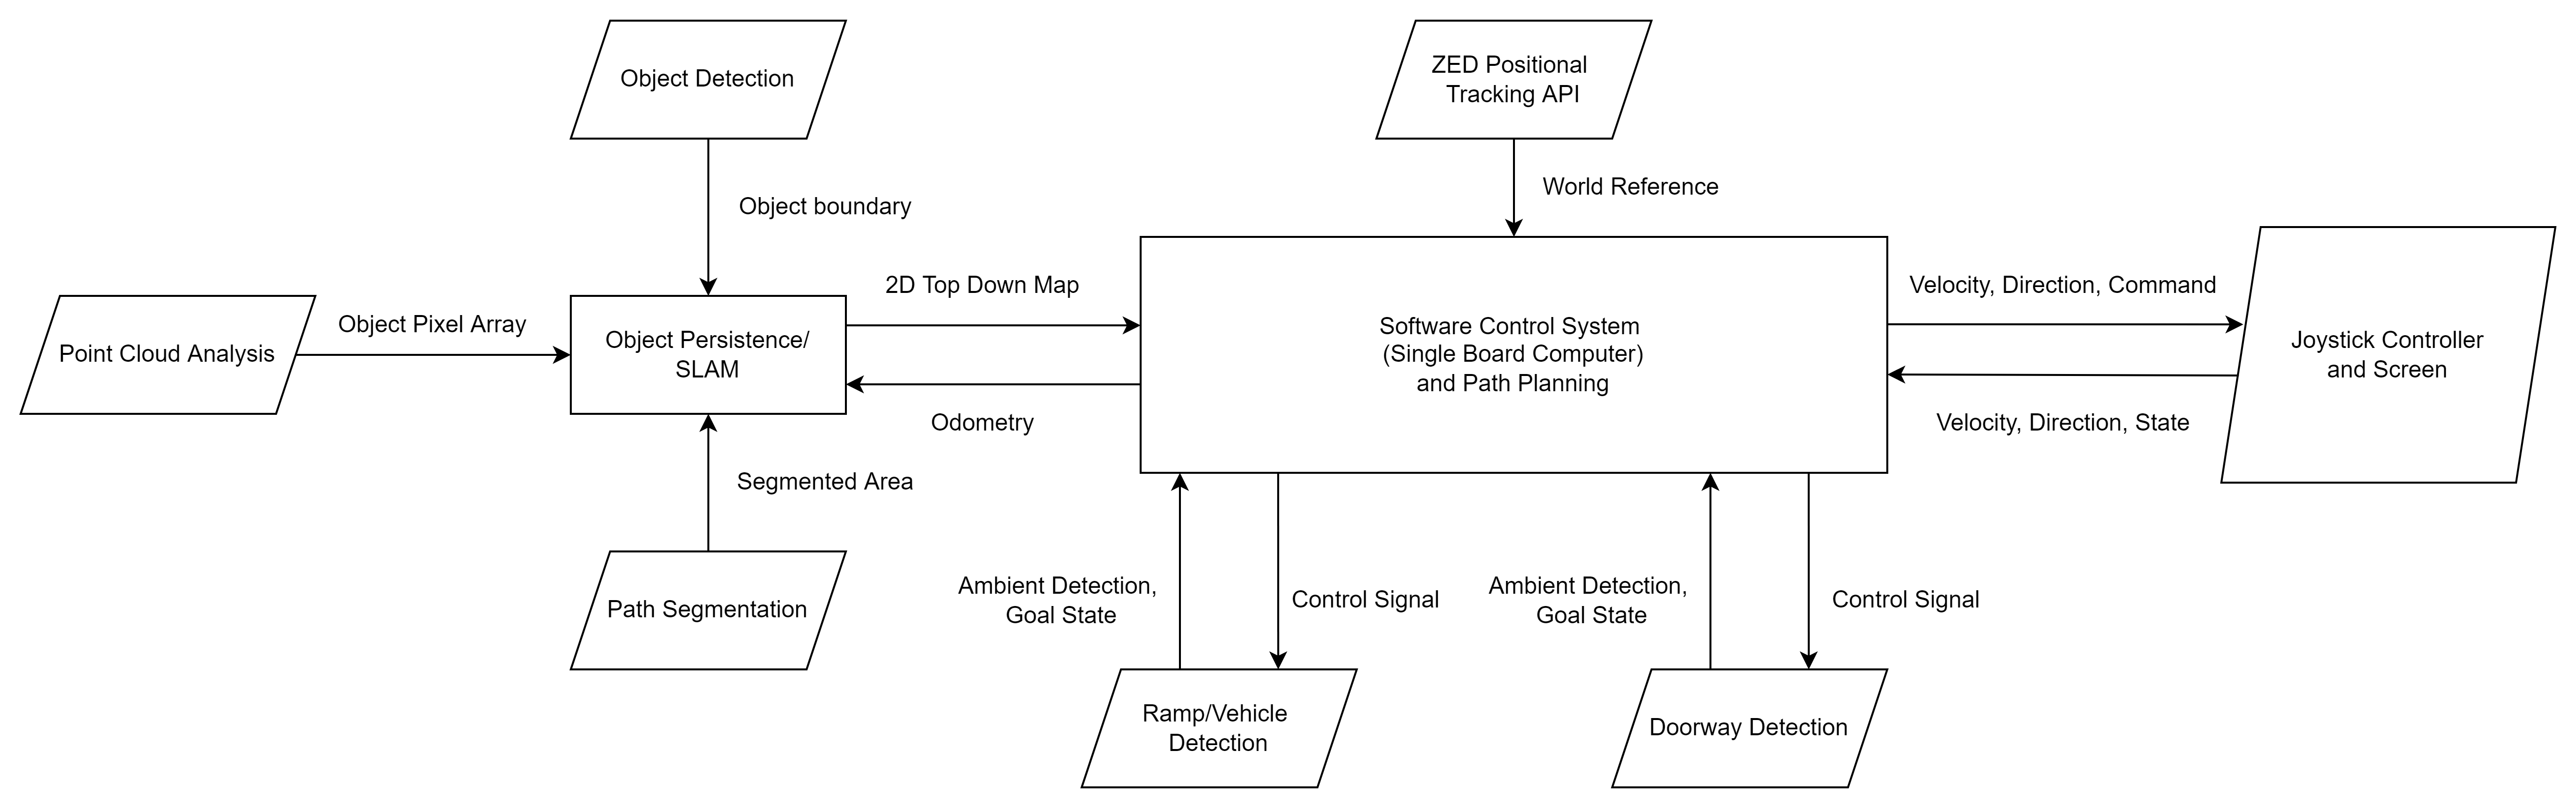
\includegraphics[width=\linewidth]{images/top_level_software_pipeline.png}
    \caption{Block diagram for future smart wheelchair system (drawn by Avinash Sudhakaran)}
    \label{fig:top_level_software_pipeline}
\end{figure}

%These systems would work by running detection algorithms
%in the background, and prompting the user to enter fully autonomous navigation using a button
%if a valid ramp or doorway was detected. These systems would then send a goal state to the
%software control system, which would perform path planning using the occupancy map and
%drive the wheelchair to this location before resuming semi-autonomous control.

% add flowchart?
% outdoor vs indoor mode
% software design - ROS and backbone
% control interface with hardware
% integration with odometry and sensors API

Once this occupancy map is built, it is passed to the software control system and used to determine
a safe speed and direction for the wheelchair using user input.
A proof-of-concept assistive control system was developed in this thesis using VFH+,
but a more robust solution would likely be required for a final implementation. The wheelchair has
two modes of operation for fully autonomous control, which are ramp/vehicle navigation (Nicolas Lee)
and doorway navigation (Avinash Sudhakaran). These modes of operation will require the user to
press a button to begin autonomous navigation when a valid ramp or doorway is detected.
These systems will send a goal pose to the software control system, which plans a safe path
using the occupancy map and drives the wheelchair to this pose. Once this has been performed,
semi-autonomous wheelchair control can resume.

To communicate between different software components, a publish/subscribe architecture
is proposed. Using a framework such as ROS (robot operating system), each component would
be defined as a node. These nodes can subscribe to other nodes to recieve data,
and publish data to a topic (recieved by other nodes) once processed. ROS supports Python and C++, which would allow
high-performance components in C++ and prototype or machine learning components in Python
to communicate. An advantage of this approach is that interfaces between nodes
are well defined, which speeds up development when multiple project students
are working on the same system.

System resources must be considered when designing a large system with many software components.
If too many processes are using the CPU or GPU accelerator, the performance of the system
will be impacted. In particular, an AI accelerator may not have enough memory or compute capability to run many complex
models at once. One way to improve the performance of the AI accelerator would be to use a shared-backbone model
architecture, which is used by Hybridnets and YOLOP. In this architecture, a complex model backbone
is used to generate image features before several smaller `heads' utilise these features for different purposes.
This would allow several models (e.g. obstacle detection, drivable area detection, doorway detection)
to run at once with only a small performance impact.
% TODO cite ROS

To communicate with the wheelchair hardware, an interface between the software control system and the
input controller/joystick controller must be implemented. The simplest way to implement this
interface would be to use a USB serial port to communicate between the microcontroller and
SBC (single board computer), with packets of data sent between the machines.
The input controller would send information such as joystick position,
seat position, and operation mode (indoor or outdoor) to the SBC. The SBC would relay back the
desired velocity and direction of the wheelchair. Additional low-bandwidth sensors, such as
1D ultrasonic sensors or wheel odometry sensors, could interface with the input controller
which would relay this information back to the SBC. The input controller would validate
the desired velocity and direction of the wheelchair before sending this information
to the motor controller, allowing it to override the SBC in the case of a software failure.

A secondary driving dataset could be collected once the input controller has been integrated into
the software control system. This driving dataset would contain joystick data and other wheelchair data
as well as the \texttt{svo} files used to record data from the ZED Mini. A simple method of storing joystick
data would be to use a csv file; alternatively, a more complex data format such as HDF5 could be used
to compress this data and store it in a binary format.

This thesis has involved implementation and testing
of various components of smart wheelchair technology. The future work detailed in
this section shows the steps needed to move from this initial research to a complete
smart wheelchair system, which can improve the safety and independence of wheelchair users.

%The positional tracking API is a high-level interface that estimates the pose of the wheelchair,
%however does not allow sensor fusion from additional sensors outside of the ZED Mini.
%One way to integrate wheel odometry sensors into the positional tracking system would
%be to use the sensors API to retrieve raw sensor data and a Kalman filter to eliminate sensor noise.


%Future work of this project involves remaining technical progress detailed in the methodology,
%and the final thesis write-up.
%Once the desired RGB-D and Lidar sensors have been procured, they will be mounted to the wheelchair
%in a secure manner and used to collect a second driving dataset around Curtin university.

%Scene recognition algorithms such as DeepLabv3 and Hybridnet
%had some difficulty identifying features of our dataset. This is likely a problem with domain adaptation,
%as the original datasets used to train these models did not include pedestrian walkways or vehicles.
%Transfer learning will be explored to improve the performance of these
%models, by training them on existing supervised driving datasets.
%Additionally, labelling of our driving dataset (using platforms such as Roboflow or V7 Labs)
%or generation of a simulated dataset will be considered.

%To improve the speed of these algorithms, GPU video encoding and post-processing will be explored.
%Maximising hardware acceleration is important for the final wheelchair hardware, as the embedded hardware will have fewer
%computational resources.

%Further evaluation and design of assistive control algorithms will ensure safe operation of the wheelchair.
%VFH+ showed promising results, however does not grant the user full control of the wheelchair
%in some scenarios and may require some modification. A basic 2D simulation environment will be created
%to model shared control between the autonomous system and the user, which will allow further tuning
%of the algorithm.

%Final integration of the autonomous system with the remaining wheelchair hardware
%will allow the demonstration of the overall system and enable direct user feedback about its performance.
%This integration will involve the development of a protocol between the wheelchair microcontroller and the compute
%element, as well as delivery of the necessary power to all components of the wheelchair.
%However, it should be noted that this final integration will be reliant on the work of other thesis students.

% Training algorithms on datasets
% Performance improvement - MMDetection or multithreaded encoder/decoder?
% Simulation environment
% Final hardware integration
% Measure kinematics
